\documentclass[12pt, a4paper]{article}

\usepackage[czech,shorthands=off]{babel}
\usepackage{lmodern}
\usepackage[utf8]{inputenc}
\usepackage[T1]{fontenc}
\usepackage[pdftex]{graphicx}
\usepackage{amsmath}
\usepackage[hidelinks,unicode]{hyperref}
\usepackage{float}
\usepackage{listings}
\usepackage{tikz}
\usepackage{xcolor}
\usepackage{tabularx}
\usepackage[final]{pdfpages}
\usepackage{syntax}


\definecolor{mauve}{rgb}{0.58,0,0.82}
\usetikzlibrary{shapes,positioning,matrix,arrows}

\newcommand{\img}[1]{(viz obr. \ref{#1})}

\definecolor{pblue}{rgb}{0.13,0.13,1}
\definecolor{pgreen}{rgb}{0,0.5,0}
\definecolor{pred}{rgb}{0.9,0,0}
\definecolor{pgrey}{rgb}{0.46,0.45,0.48}

\usepackage[sorting=nyt,style=ieee]{biblatex}
\addbibresource{literatura.bib}

\lstdefinestyle{flex}{
    frame=tb,
    aboveskip=3mm,
    belowskip=3mm,
    showstringspaces=false,
    columns=flexible,
    basicstyle={\small\ttfamily},
    numbers=none,
    numberstyle=\tiny\color{black},
    keywordstyle=\color{black},
    commentstyle=\color{black},
    stringstyle=\color{black},
    breaklines=true,
    breakatwhitespace=true,
    tabsize=3
}

\lstset{
    frame=tb,
    language=XML,
    aboveskip=3mm,
    belowskip=3mm,
    showstringspaces=false,
    columns=flexible,
    basicstyle={\small\ttfamily},
    numbers=none,
    numberstyle=\tiny\color{gray},
    keywordstyle=\color{blue},
    commentstyle=\color{pgreen},
    stringstyle=\color{mauve},
    breaklines=true,
    breakatwhitespace=true,
    tabsize=3
}


\let\oldsection\section
\renewcommand\section{\clearpage\oldsection}

\begin{document}
	% this has to be placed here, after document has been created
	% \counterwithout{lstlisting}{chapter}
	\renewcommand{\lstlistingname}{Ukázka kódu}
	\renewcommand{\lstlistlistingname}{Seznam ukázek kódu}
    \begin{titlepage}

        \centering

        \vspace*{\baselineskip}
        \begin{figure}[H]
        \centering
        
\includegraphics[width=7cm]{img/fav-logo.jpg}
        \end{figure}

        \vspace*{1\baselineskip}

        \vspace{0.75\baselineskip}

        \vspace{0.5\baselineskip}
        {Semestrální práce z předmětu KIV/NET}

        {\LARGE\sc Aplikace pro sledování obchodního portfólia s kryptoměnami \\}

        \vspace{4\baselineskip}

        \vspace{0.5\baselineskip}

        {\sc\Large Stanislav Král \\}
        \vspace{0.5\baselineskip}
        {A20N0091P}

        \vfill

        {\sc Západočeská univerzita v Plzni\\
        Fakulta aplikovaných věd}

    \end{titlepage}


    % TOC
    \tableofcontents
    \pagebreak

\section{Zadání práce}
Zadáním práce je vytvořit aplikaci určenou ke sledování obchodního portfólia s kryptoměnami pomocí frameworku .NET 5.0, kdy aplikace bude nabízet grafické rozhraní pro její ovládání. Aplikace musí splňovat následující body:

\begin{itemize}
    \item možnost vytvořit portfólia, do kterých budou členěněny jednotlivé transakce (jedno portfólio může obsahovat pouze transakce v jedné fiat měně)
    \item jednotlivé transakce budou obsahovat informaci o nákupní či prodejní ceně za jednu minci kryptoměny, počet mincí, kterých se obchod týkal, datum uskutečnění obchodu a poplatek za jeho zprostředkování
    \item možnost zobrazit si celkový zisk či ztrátu portfólia 
    \item možnost zobrazit si zisk či ztrátu na úrovni jednotlivých transakcí
    \item možnost zobrazit si procentuální složení daného portfólia
    \item možnost získat aktuální kurz vybrané kryptoměny ze zdroje dostupného přes veřejně dostupné REST API 
    \item vhodně navržená architektura umožující možnost jednoduchou výměnu datové vrstvy či zdroje aktuálního kurzu
\end{itemize}

    
\section{Sledování obchodního portfólia s kryptoměnami}

Obchodování kryptoměň spočívá v nákupu a prodeji kryptoměn na burzách za účelem zisku, kdy obchodník chce prodat kryptoměny za vyšší částku než je nakoupil. Je typické, že takový obchodník provádí velké množství obchodů (až několik týdně) a i přesto, že burzy s kryptoměnami sice poskytují přehled historie uskutečněných transakcí, tak tento přehled nebývá často dostatečně obsáhlý a některé informace, jako například zisk či ztráta, se v něm nezobrazují. Dále je také časté, že obchodníci používají k obchodování více než jednu burzu, a tak vzniká potřeba nějaké služby či aplikace, ve které by byly transakce ze všech burz uložené, a která by nabízela jednoduché a společné rozhraní pro všechny burzy. Od takové služby je vyžadovaný i kvalitní přehled zobrazující aktuální výkon obchodování a celkovou hodnotu výdělku či ztráty. Mezi nejpopulárnější kryptoměnové burzy patří například \textit{Coinbase} či \textit{Binance}. 

Za předpokladu existence takové aplikace by jejím dalším využitím, jelikož sdružuje transakce ze všech burz, bylo použití při vyplňování daňového přiznání, kdy je velmi výhodné, že aplikace zobrazuje všechny obchodníkovy transakce včetně zisku či ztráty.  

Aplikací, které se zaměřují na sledování obchodního portfólia s kryptoměnami existuje několik, kdy mezi ty nejpoužívanější patří Blockfolio\cite{blockfolio2021} (Android a iOS), Delta\cite{delta2021} (Android a iOS) a Moonitor\cite{moonitor2021} (macOS, Windows a Linux). Tyto aplikace splňují požadavek přehledného zobrazení výnosnosti obchodování i na úrovni jednotlivých transakcí, avšak během jejich používání můžou často vzniknout nové požadavky specifické danému uživateli, jako například možnost importu transakcí z API nějaké méně známé burzy či jiný výpočet celkového zisku portfólia, které do aplikace pravděpodobně nikdy nebudou zapracovány. Řešením pro technicky zdatné uživatele by bylo si takovou aplikaci navrhnout a napragramovat, avšak vytváření architektury a základní logiky pro správu a sledování portfólia (zádávní transakcí a jejich přehled) pro ně může být časově náročné a tudíž odrazující. 

\begin{figure}[!ht]
\centering
{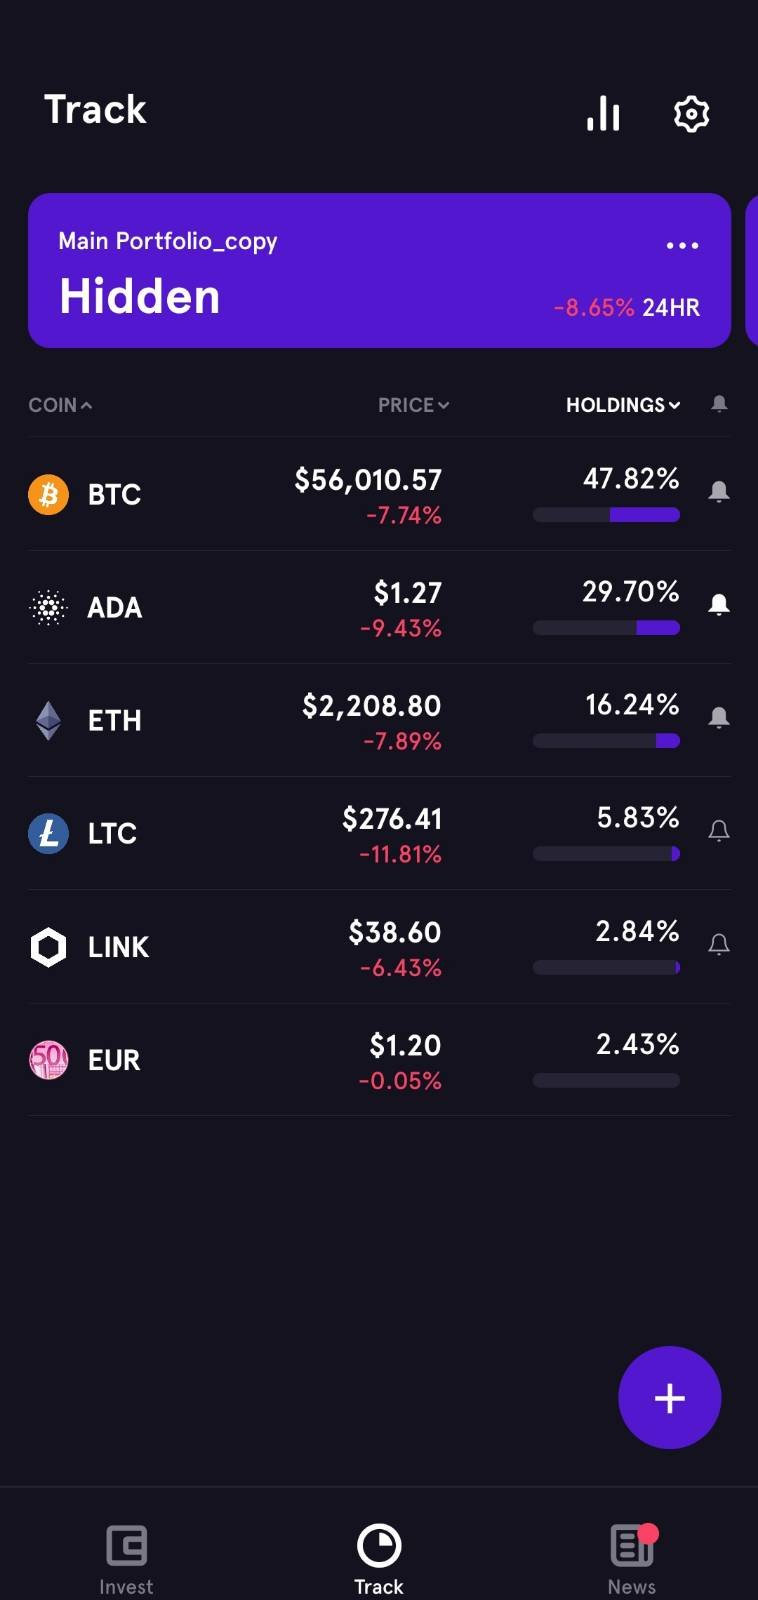
\includegraphics[width=5.5cm]{img/blockfolio.png}}
\caption{Mobilní aplikace Blockfolio umožňující sledovat kryptoměnové portfólio}
\label{fig:simple-vrp-czech}
\end{figure}

\section{Datový zdroj s aktuálním kurzem kryptoměn}

Pro vývoj aplikace určené ke sledování obchodního portfólia s kryptoměnami je třeba nalézt vhodný zdroj dat, který bude využíván k získávání aktuálního kurzu sledovaných kryptoměn. Mezi hlavní požadavky na takový datový zdroj je jeho dostupnostie jednoduchost rozhraní a množina podporovaných kurzů. Ideálním zdrojem je tedy takový zdroj, který poskytuje aktuální i historický kurz na všech burzách prostřednictvím REST API bez nutnosti registrace.

\subsection{Webový zdroj CoinGecko}
Aktuální i historický kurz drtivé většiny všech existujících kryptoměn bez nutnosti registrace nabízí pomocí REST rozhraní webová služba CoinGecko\cite{coingecko2021}. Jediným omezením tohoto API je počet provedených požadavků za minutu, který je stanoven na 100, což je pro aplikaci určenou ke sledování kryptoměnového portfólia více než dostačující.

\begin{lstlisting}
$ curl -X GET "https://api.coingecko.com/api/v3/simple/price?ids=bitcoin&vs_cur
rencies=usd" -H  "accept: application/json"

{
  "bitcoin": {
    "usd": 56224
  }
}
\end{lstlisting}

\section{Výběr databáze pro implementaci datové vrstvy aplikace}

Jelikož vytvářená aplikace není určená pro použití vícero uživateli najednou, ale pouze pro jednoho uživatele na jednom zařízení, tak pro ukládání dat aplikace je vhodná lokální databáze. 

V úvahu připadá ukládat portfólia a transakce ve formátu JSON či XML přímo na souborový systém, ale z důvodu relace M:N mezi portfólii a kryptoměnami nejsou tyto typy databází příliš vhodné. Jako lepší volba tedy jeví nějaká relační databáze, např. SQLite, která je často používána při tvorbě desktopových aplikací a ukládá se ve formě jednoho souboru na souborový systém zařízení.

\section{Framework pro grafické rozhraní}
\textit{Frontend realizovaný pomocí Blazor frameworku, zabalený do Electron wrapperu}


\printbibliography


\end{document} 
